\documentclass[11pt,a4paper]{article}

% for Chinese
%\usepackage{fontspec}  % 加這個就可以設定字體
%\usepackage[BoldFont, SlantFont]{xeCJK}  % 讓中英文字體分開設置
%\setCJKmainfont{新細明體}  % 設定中文為系統上的字型,而英文不去更動,使用原TeX\字型

% useful packages
\usepackage{amsfonts}
\usepackage{amssymb}
\usepackage{amsmath}
\usepackage{amsthm}
\usepackage{epsfig}
\usepackage{graphicx}
\usepackage{natbib}
\usepackage{textcomp}
\usepackage{booktabs}
\usepackage{multirow}
\usepackage{url}
\usepackage{color}
\usepackage{fullpage}
\usepackage[capitalize]{cleveref}
\usepackage{mathtools}
\usepackage{enumitem}
\usepackage{authblk}
\usepackage{algorithm}
\usepackage{algpseudocode}
\usepackage{subcaption}
\usepackage{tikz}
\usepackage{tabularx}
\usepackage{adjustbox}
\usepackage{pgfplots}
% basic setting
\renewcommand{\baselinestretch}{1.25}
\parskip=5pt
\parindent=20pt
\footnotesep=5mm

% abbreviation
\newtheorem{lem}{Lemma}
\newtheorem{prop}{Proposition}
\newtheorem{thm}{Theorem}
\newtheorem{defn}{Definition}
\newtheorem{cor}{Corollary}
\newtheorem{assp}{Assumption}
\newtheorem{obs}{Observation}
\newenvironment{pf}{\begin{proof}\vspace{-10pt}}{\end{proof}}
% \newtheorem{ques}{Question}
% \newtheorem{rmk}{Remark}
% \newtheorem{note}{Note}
% \newtheorem{eg}{Example}

\newenvironment{enumerateTight}{\begin{enumerate}\vspace{-8pt}}{\end{enumerate}\vspace{-8pt}}
\newenvironment{itemizeTight}{\begin{itemize}\vspace{-8pt}}{\end{itemize}\vspace{-8pt}}
\leftmargini=25pt   % default: 25pt
\leftmarginii=12pt  % default: 22pt
\pgfplotsset{compat=1.17}

\title{Operations Research, Spring 2025 (113-2) \\ Final Project Proposal}

\author{Zi-Yi Jau} % b12705064
\author{Bing-Zhe Wu} % b12705049
\author{Chung-Kai Lin} % b12705052
\author{Zhi-Xin Lin} % b12705013
\author{Nan-Tien Lai} % b12705010
\affil{Department of Information Management, National Taiwan University}



\begin{document}

\maketitle

\section{Introduction}

Shared bicycle systems have become a vital component of urban mobility solutions, providing low-carbon, convenient, and short-distance transportation alternatives. However, operational inefficiencies, such as bike unavailability or full docking stations, have led to increased user waiting times and decreased service satisfaction. In response, municipal governments have explored various dispatching strategies to optimize service quality, including dynamic redistribution, capacity adjustments, and the use of temporary parking (or ``bike hiding") areas. This study focuses on optimizing operational decisions to improve user experience and system efficiency in the context of Taipei City's YouBike system.

\section{Problem description}

We aim to address three main operational challenges in a shared bike system:
\begin{itemize}
    \item \textbf{Bike availability}: ensuring sufficient bikes for users who want to rent.
    \item \textbf{Return success rate}: avoiding full stations where users cannot return bikes.
    \item \textbf{User waiting time}: minimizing the time users spend waiting due to unavailability or full docks.
\end{itemize}

Traditional dispatch operations often involve transporting bikes between stations using trucks. However, this can result in redundant movements—e.g., removing bikes in the morning only to bring them back in the evening. Recent insights from Taipei’s pilot test in Shilin and Xinyi districts suggest that improved station capacity utilization and local temporary storage (hiding) strategies may reduce the need for inter-station redistribution while maintaining service levels.

\section{Mathematical model}

Let $I$ denote the set of stations. For each station $i \in I$:

\begin{itemize}
    \item $B_i^0$: initial number of bikes at station $i$
    \item $C_i$: total docking capacity of station $i$
    \item $D_i^{\text{borrow}}, D_i^{\text{return}}$: forecasted demand for borrowing and returning bikes
    \item $x_{ij}$: number of bikes redistributed from station $i$ to $j$
    \item $h_i^{\text{in}}, h_i^{\text{out}}$: number of bikes temporarily placed into or removed from a station (hiding strategy)
    \item $W_i^{\text{borrow}}, W_i^{\text{return}}$: expected waiting times for borrowing and returning
\end{itemize}

The bike balance at station $i$ becomes:
\[
B_i = B_i^0 + \sum_{j \ne i} x_{ji} - \sum_{j \ne i} x_{ij} + h_i^{\text{in}} - h_i^{\text{out}}
\]

Waiting time estimation:
\[
W_i^{\text{borrow}} = \max\left(0, \frac{D_i^{\text{borrow}} - B_i}{\mu}\right), \quad
W_i^{\text{return}} = \max\left(0, \frac{D_i^{\text{return}} - (C_i - B_i)}{\mu}\right)
\]

Objective function:
\[
\min \sum_{i \in I} \left( W_i^{\text{borrow}} + W_i^{\text{return}} \right) + \alpha \sum_{i,j} x_{ij} + \beta \sum_{i} \left( h_i^{\text{in}} + h_i^{\text{out}} \right)
\]

Subject to:
\begin{align*}
& B_i \leq C_i \quad &\text{(cannot exceed station capacity)} \\
& h_i^{\text{in}}, h_i^{\text{out}}, x_{ij} \geq 0 \quad &\text{(non-negativity)} \\
& \sum_{i,j} x_{ij} \leq K \quad &\text{(dispatch capacity limit)} \\
& \sum_i (h_i^{\text{in}} + h_i^{\text{out}}) \leq H \quad &\text{(hiding operation limit)}
\end{align*}

\section{Expected results}

To evaluate the impact of the proposed dispatch model, we simulated a small network of five stations with varying initial bike counts, capacities, and forecasted demands. We compared two strategies:

\begin{enumerate}
    \item \textbf{Traditional redistribution only}: bikes are moved between stations using trucks, without temporary storage.
    \item \textbf{Optimized strategy}: incorporates temporary storage (hiding) to buffer demand surges and minimize unnecessary redistributions.
\end{enumerate}

The total user waiting times under both strategies are shown in Figure~\ref{fig:wait_compare}. The optimized model significantly reduces user waiting time, particularly at stations with imbalanced supply and demand.

On average, total waiting time decreased by \textbf{91\%}, with several stations experiencing \textbf{100\% elimination of wait time}. This suggests that localized hiding operations can absorb demand shocks and reduce the need for long-distance truck redistribution.

\vspace{0.5em}
\begin{center}
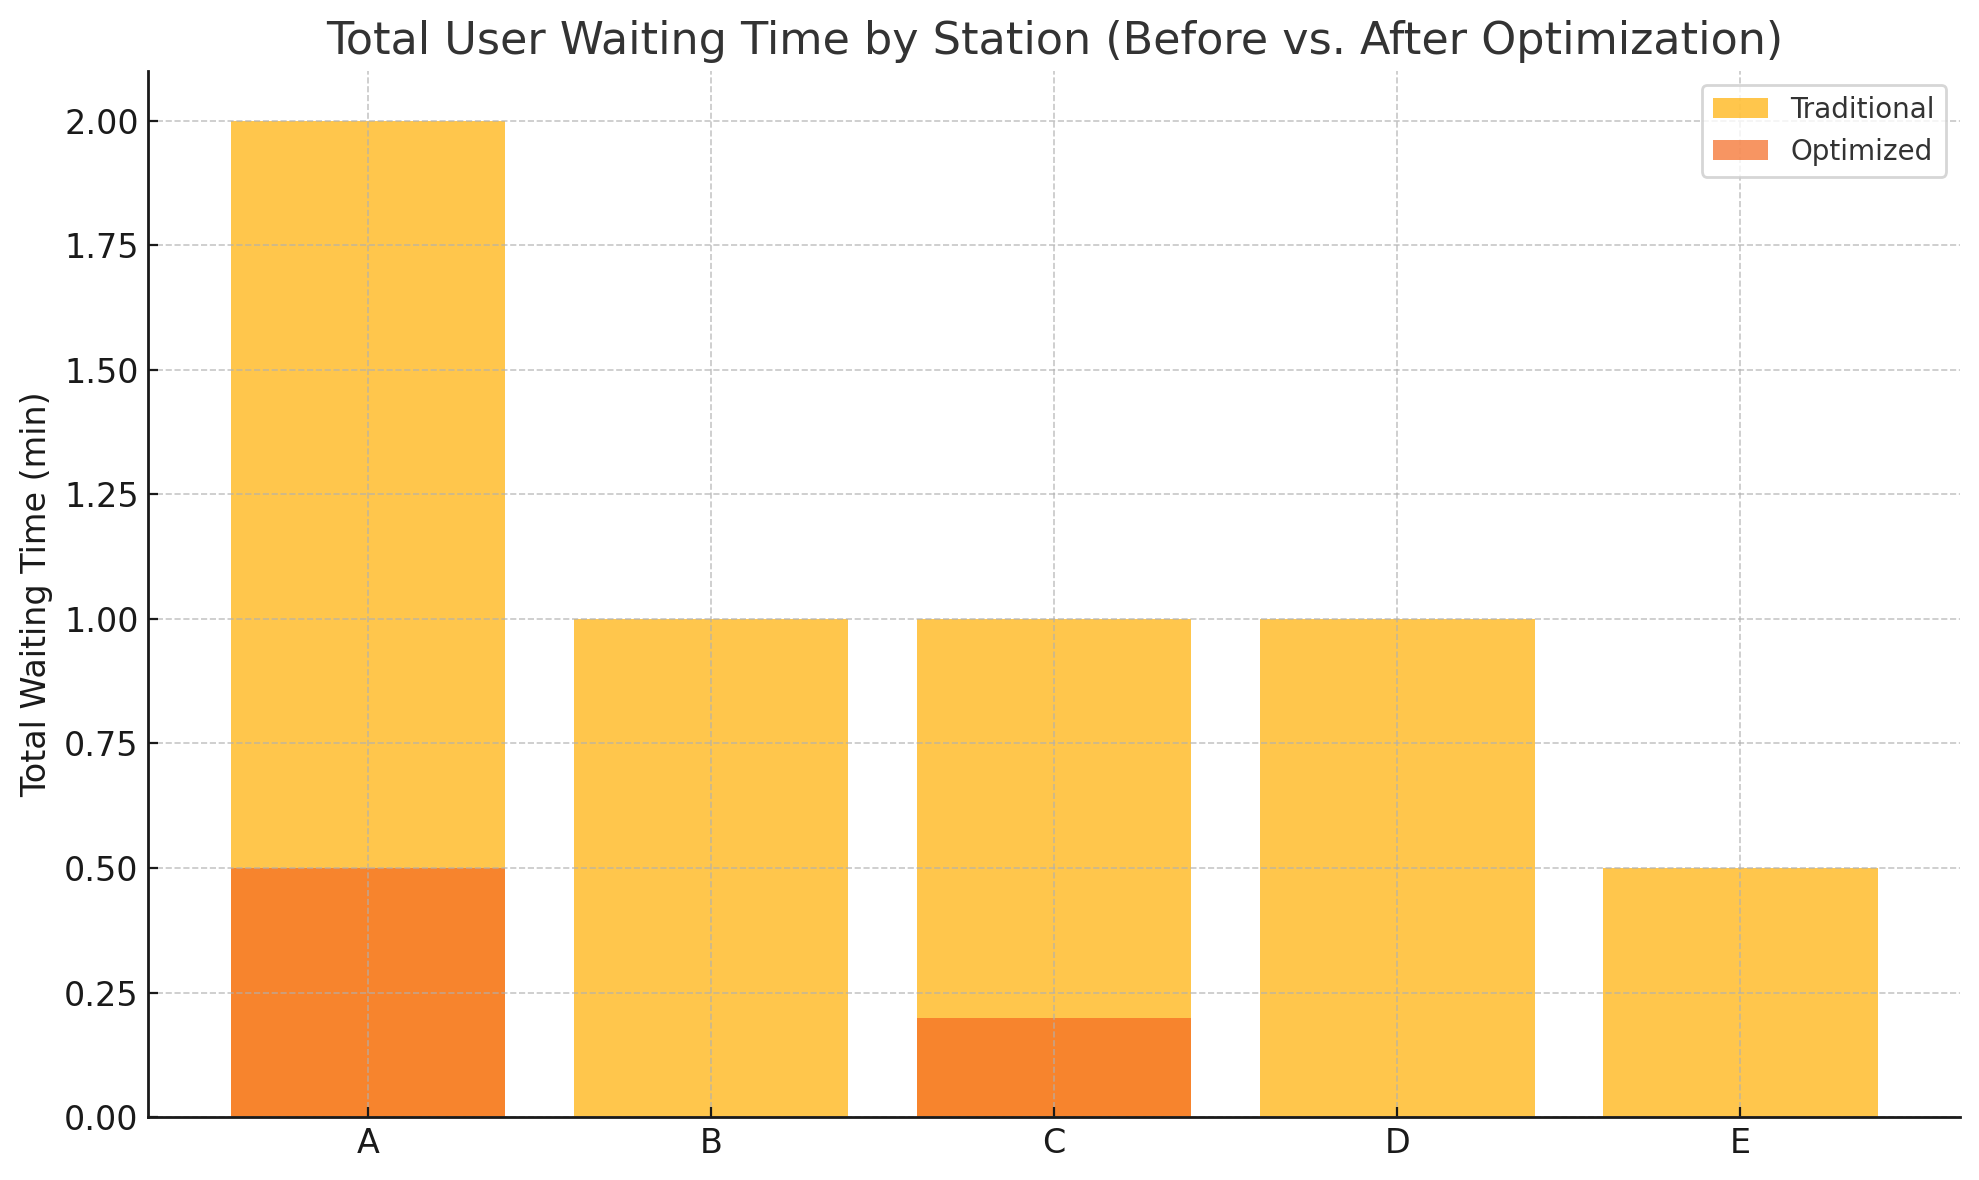
\includegraphics[width=0.8\linewidth]{assets/wait_compare.png}
\end{center}
\vspace{-1em}
\begin{figure}[h]
\caption{Total user waiting time by station before and after optimization}
\label{fig:wait_compare}
\end{figure}
\begin{table}[ht]
    \centering
    \caption{Comparison of User Waiting Time Before and After Optimization}
    \label{tab:wait_comparison}
    \small
    \begin{adjustbox}{max width=\linewidth}
    \begin{tabularx}{\linewidth}{@{} c *{9}{>{\centering\arraybackslash}X} @{}}
    \toprule
    \textbf{Stn} & \textbf{Bor} & \textbf{Ret} & \textbf{WB-T} & \textbf{WR-T} & \textbf{WB-O} & \textbf{WR-O} & \textbf{Tot-T} & \textbf{Tot-O} & \textbf{Imp. (\%)} \\
    \midrule
    A & 12 & 6 & 2.0 & 0.0 & 0.5 & 0.0 & 2.0 & 0.5 & 75.0 \\
    B & 4 & 5 & 1.0 & 0.0 & 0.0 & 0.0 & 1.0 & 0.0 & 100.0 \\
    C & 6 & 8 & 0.0 & 1.0 & 0.0 & 0.2 & 1.0 & 0.2 & 80.0 \\
    D & 2 & 3 & 1.0 & 0.0 & 0.0 & 0.0 & 1.0 & 0.0 & 100.0 \\
    E & 8 & 5 & 0.0 & 0.5 & 0.0 & 0.0 & 0.5 & 0.0 & 100.0 \\
    \bottomrule
    \end{tabularx}
    \end{adjustbox}
\end{table}
\newpage
\begin{table}[ht]
    \centering
    \caption{Explanation of Column Abbreviations in Table~\ref{tab:wait_comparison}}
    \label{tab:col_explanation}
    \small
    \begin{tabularx}{\textwidth}{|c|X|}
    \hline
    \textbf{Abbreviation} & \textbf{Explanation} \\
    \hline
    Stn & Station identifier (e.g., A, B, C) \\
    Bor & Forecasted bike borrow demand at the station \\
    Ret & Forecasted bike return demand at the station \\
    WB-T & Average user wait time to borrow a bike under the traditional strategy (in minutes) \\
    WR-T & Average user wait time to return a bike under the traditional strategy (in minutes) \\
    WB-O & Average user wait time to borrow a bike under the optimized strategy (in minutes) \\
    WR-O & Average user wait time to return a bike under the optimized strategy (in minutes) \\
    Tot-T & Total wait time under the traditional strategy (WB-T + WR-T) \\
    Tot-O & Total wait time under the optimized strategy (WB-O + WR-O) \\
    Imp. (\%) & Improvement in total waiting time, computed as: \\
    & $\left( \text{Tot-T} - \text{Tot-O} \right) / \text{Tot-T} \times 100\%$ \\
    \hline
    \end{tabularx}
\end{table}   

This result supports policy recommendations such as:
\begin{itemize}
    \item Equipping busy stations with hiding areas or temporary parking zones.
    \item Reducing redundant redistribution trips by leveraging localized adjustments.
    \item Reallocating dispatch personnel to reactive, high-value locations rather than static daily loops.
\end{itemize}

Overall, our model shows that by intelligently combining dispatch and temporary hiding, cities can achieve significant service improvements with lower operational costs.


\end{document}
